\documentclass[]{article}
\usepackage{subfiles}
\usepackage[pdftex]{graphicx} % remove pdftex if you are not compiling to pdf
%\usepackage{subfig}
\usepackage{float}
\graphicspath{{./figures/}}
\DeclareGraphicsExtensions{.pdf,.png,.jpg}
\usepackage[caption=false]{subfig}
\usepackage{xcolor}
\usepackage{booktabs}
\usepackage[%
    style=phys
    ,backend=biber
    ,natbib=true
    ,maxbibnames=6
    ,biblabel=brackets
    %,giveninits=trueb
    %,abbreviate=false
    ,doi=false 
    ,url=false 
    ,isbn=false
    ,eprint=false
    %,block=space
    %,backref=true
    %,backrefstyle=two
    %,hyperref=true
]
{biblatex}
\addbibresource{sample.bib}
%\usepackage{cite}
\usepackage[toc,page]{appendix}
\usepackage{amsmath}
\usepackage{enumitem}
\usepackage{lineno}
\linenumbers

\title{Measurement of Muon neutrino Charged-Current Neutral Pion Production at ICARUS}
\author{Lane Kashur}
\date{\today}

\begin{document}

\maketitle

\begin{abstract}
Begin abstract \vspace{1cm} \\

End abstract
\end{abstract}

\tableofcontents

% Sections
\subfile{sections/section1}
\subfile{sections/section2.tex}
\subfile{sections/section3.tex}
\subfile{sections/section4.tex}
\subfile{sections/section5.tex}

\section{Conclusions}

%\bibliographystyle{unsrt} % math and engineering style bibliography
%\bibliography{sample}

\printbibliography

\begin{appendices}

\section{Data Quality Cuts}
\label{appendix:dataquality}

\section{Raw Signal Processing and Calibration}
\label{appendix:sigandcalib}

\section{Machine Learning Reconstruction}
\label{appendix:mlreco}
In this section, neutrino event reconstruction is discussed.  For information on raw signal processing and calibration, see Appendix \ref{appendix:sigandcalib}.
Reconstruction of neutrino events is handled by the end-to-end, machine-learning based reconstruction chain known as SPINE (Scalable Particle Imaging with Neural Embeddings) \cite{spinepaper}.  As input, SPINE takes an image of 3D charge depositions within the detector, which is then operated on by a series of neural networks to carry out point classification and formation of particle and interaction objects.

\begin{figure}[H]
    \center
    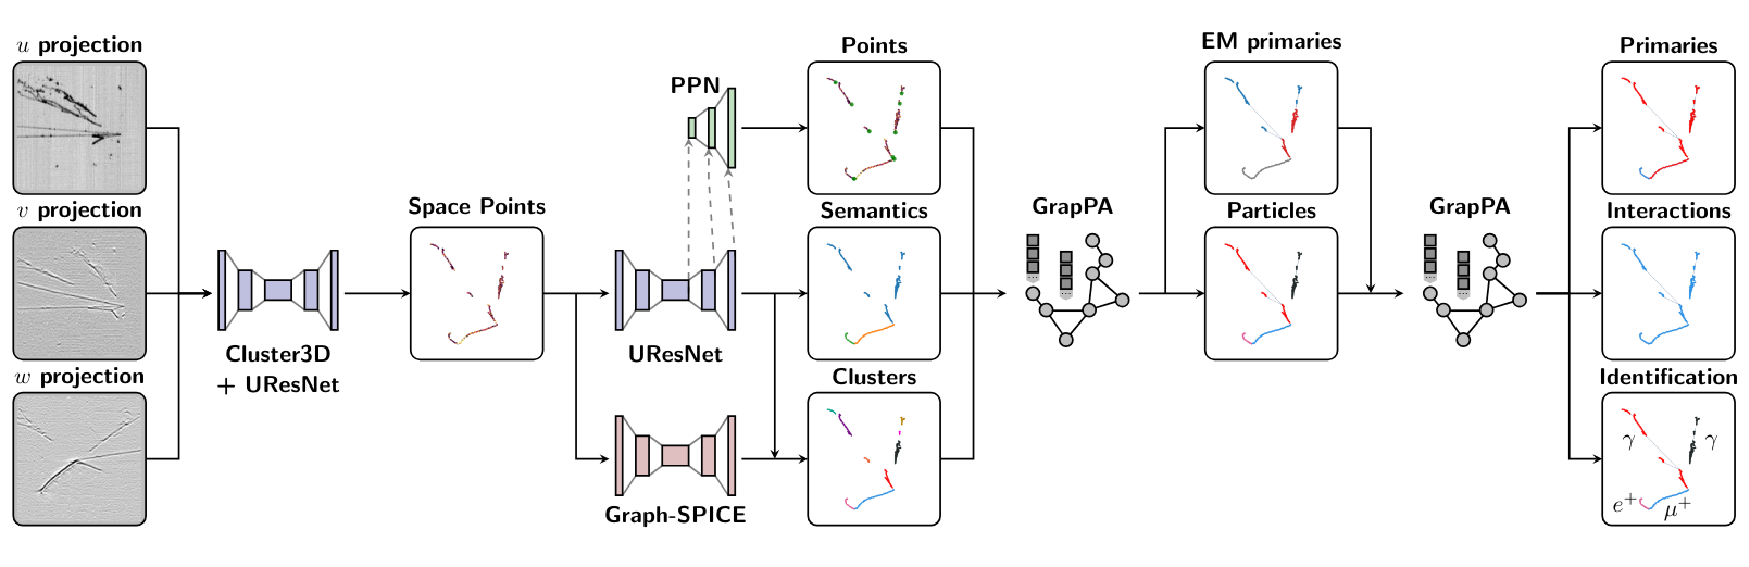
\includegraphics[width=0.90\textwidth]{figures/spinechain.pdf}
    \caption[text]{The SPINE reconstruction chain.}
    \label{fig:spinechain}
\end{figure}

\subsection{Point Classification}
Point classification refers to the classification of 3D space points into abstract particle classes and the identification of points of interest.  Convolution neural networks (CNNs) are used for these tasks, beginnining with the removal of tomographic reconstruction artifacts by the 

\subsection{Formation of Particles and Interactions}

\subsection{Post-Processors}

\end{appendices}

\end{document}